\documentclass[11pt, oneside, titlepage]{article}
\usepackage[letterpaper, margin=2cm]{geometry}
\usepackage{MATH517}
\usepackage{Calculus}

\title{MATH 517 Finite Differences Homework 4}
\author{Caleb Logemann}

\begin{document}
\maketitle

%\lstinputlisting[language=Matlab]{H01_23.m}
\begin{enumerate}
    \item % #1
        Consider the Leapfrog method
        \[
            U^{n+1} = U^{n−1} + 2k f(U^n)
        \]
        applied to the test problem $u′ = \lambda u$.
        The method is zero-stable and second order accurate, and hence convergent.
        If $\lambda < 0$ then the true solution is exponentially decaying.

        On the other hand, for $\lambda < 0$ and $k > 0$ the point $z = k\lambda$ is never in the
        region of absolute stability of this method,
        and hence the numerical solution should be growing exponentially for any
        nonzero time step.
        (And yet it converges to a function that is exponentially decaying.)

        Suppose we take $U^0 = \eta$, use Forward Euler to generate $U^1$, and
        then use the midpoint method for $n = 2, 3, \cdots$.
        Work out the exact solution $U^n$ by solving the linear difference
        equation and explain how the apparent paradox described above is resolved

        We know that $U^0 = \eta$ and
        $U^1 = U^0 + k \lambda U^0 = (1 + k\lambda)\eta$ by the Euler method.
        We also know that the solution is governed by the difference equation
        \[
            U^{n+1} - 2k\lambda U^n - U^{n-1} = 0
        \]
        We know that solutions to this difference equation are solutions of the
        following equation
        \[
            \zeta^2 - 2k\lambda \zeta - 1 = 0
        \]

        Using the quadractic formula solutions to this equation can be found
        \begin{align*}
            \zeta &= \frac{2k\lambda \pm \sqrt{4(k\lambda)^2 - 4(1)(-1)}}{2} \\
                  &= k\lambda \pm \sqrt{(k\lambda)^2 + 1} \\
        \end{align*}

        This implies that the general solution to the linear difference
        equation is of the form
        \[
            U^n = c_1(k\lambda + \sqrt{(k\lambda)^2 + 1})^n + c_2(k\lambda - \sqrt{(k\lambda)^2 + 1})^n
        \]

        Using the initial conditions that $U^0 = \eta$ and
        $U^1 = (1 + k\lambda)\eta$, it is possible to solve for the constants
        $c_1$ and $c_2$.

        \begin{align*}
            \eta &= c_1 + c_2 \\
            c_2 &= \eta - c_1 \\
            (1 + k\lambda)\eta &= c_1(k\lambda + \sqrt{(k\lambda)^2 + 1}) + c_2(k\lambda - \sqrt{(k\lambda)^2 + 1}) \\
            (1 + k\lambda)\eta &= c_1(k\lambda + \sqrt{(k\lambda)^2 + 1}) + (\eta - c_1)(k\lambda - \sqrt{(k\lambda)^2 + 1}) \\
            (1 + k\lambda)\eta &=  2c_1\sqrt{(k\lambda)^2 + 1} + \eta(k\lambda - \sqrt{(k\lambda)^2 + 1}) \\
            c_1 &= \frac{\eta(1 + \sqrt{(k\lambda)^2 + 1})}{2\sqrt{(k\lambda)^2 + 1}} \\
            c_1 &= \frac{\eta(\sqrt{(k\lambda)^2 + 1} + (k\lambda)^2 + 1)}{2(k\lambda)^2 + 2} \\
            c_2 &= \eta - \frac{\eta(\sqrt{(k\lambda)^2 + 1} + (k\lambda)^2 + 1)}{2(k\lambda)^2 + 2} \\
            c_2 &= \eta\frac{(k\lambda)^2 + 1 -\sqrt{(k\lambda)^2 + 1}}{2(k\lambda)^2 + 2} \\
        \end{align*}


    \item % #2 Done
        \begin{enumerate}
            \item[(a)]
                Find the general solution of the linear difference equation
                \[
                    U^{n+3} + 2U^{n+2} - 4U^{n + 1} - 8U^n = 0
                \]

                The general solution of the linear difference equation can be
                found by finding the roots of the following polynomial.
                \[
                    \zeta^3 + 2\zeta^2 - 4\zeta - 8
                \]
                This polynomial factors to
                \[
                    (\zeta - 2)(\zeta + 2)^2
                \]
                Thus the general solution to this linear difference equation is
                \[
                    U^n = c_1 2^n + c_2 (-2)^n + c_3 n (-2)^n
                \]

            \item[(b)]
                Determine the particular solution with initial data $U_0 = 4$,
                $U_1 = -2$, and $U_2 = 8$.

                The particular solution can be found as follows.
                \begin{align*}
                    U^0 &= 4 = c_1 + c_2 \\
                    c_1 &= 4 - c_2 \\
                    U^1 &= -2 = 2 c_1 - 2 c_2 - 2c_3 \\
                    -2 &= 2(4 - c_2) - 2 c_2 - 2 c_3 \\
                    -10 + 4 c_2 &= -2 c_3 \\
                    c_3 &= 5 - 2 c_2
                    U^2 &= 8 = 4c_1 + 4c_2 + 8c_3 \\
                    8 &= 4(4 - c_2) + 4c_2 + 8(5 - 2c_2) \\
                    8 &= 16 - 4c_2 + 4c_2 + 40 - 16c_2 \\
                    -48 &= -16c_2 \\
                    c_2 &= 3 \\
                    c_1 &= 1 \\
                    c_3 &= -1 
                \end{align*}
                Thus the particular solution is $U^n = 2^n + (3 - n)(-2)^n$.

            \item[(c)]
                Consider the iteration:
                \[
                    \begin{bmatrix}
                        U^{n+1} \\
                        U^{n+2} \\
                        U^{n+3}
                    \end{bmatrix}
                    =
                    \begin{bmatrix}
                        0 & 1 & 0 \\
                        0 & 0 & 1 \\
                        8 & 4 & 2
                    \end{bmatrix}
                    \begin{bmatrix}
                        U^n \\
                        U^{n+1} \\
                        U^{n+2}
                    \end{bmatrix}
                \]
                The matrix appearing here is the companion matrix for the
                difference equation.
                If this matrix is called $A$, then we can determine $U^n$ from
                the starting values if we know $A^n$, the nth power of $A$.
                If $A = R\Lambda R^{-1}$ is the Jordan Canonical form for the
                matrix, then $A^n = R\Lambda^n R^{-1}$.
                Determine the eigenvalues and Jordan canonical form for this
                matrix and show how this is related to the general solution
                found in (a).
                The eigenvalues of $A$ can be found by solving the following

                equation
                \begin{align*}
                    \det(A - \lambda I) &= 0
                    -\lambda^3 - 2\lambda^2 + 4\lambda + 8 &= 0
                \end{align*}
                This equation has the same solutions as the root of the
                polynomial in part (a).
                Therefore the eigenvalues are $\lambda = 2, -2, -2$.
                The Jordan Cononical form of $A$ is
                \[
                    \Lambda =
                    \begin{bmatrix}
                        2 & 0 & 0 \\
                        0 & -2 & 1 \\
                        0 & 0 & -2
                    \end{bmatrix}
                \]
                The eigenvalues correspond directly roots of the characteristic
                polynomial of the lienar difference equation.
        \end{enumerate}

    \item % #3
        Write a MATLAB script to plot the region of absolute stability of the
        4-stage Runge-Kutta method. (See example 5.13 on Page 126)

        I chose to use Mathematica instead to plot the region of absolute
        stability with the following script.
        \begin{verbatim}
Y1 = Un;
Y2 = Un + 1/2 k L Y1;
Y3 = Un +1/2 k L (Y2);
Y4 = Un + k L(Y3);
Un1 = Un + 1/6 k L(Y1 + 2(Y2) + 2(Y3) +Y4)//FullSimplify//Expand

Un+k Un L+1/2 k^2 Un L^2+1/6 k^3 Un L^3+1/24 k^4 Un L^4

(1 + k L + 1/2 (k L)^2 + 1/6 (k L)^3 + 1/24 (k L)^4)Un

p[z_]:=1 + z + 1/2 z^2 + 1/6 z^3 + 1/24 z^4
RegionPlot[Abs[p[x + I y]]<=1,{x,-5,5},{y,-5,5},Axes->True,Frame->False]
        \end{verbatim}
        \begin{center}
            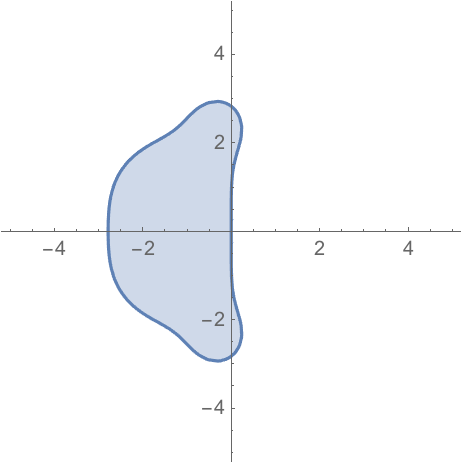
\includegraphics[scale=.5]{Figures/05_3.png}
        \end{center}

    \item % #4
        \begin{enumerate}
            \item[(a)]
                We know that the stages of a Runge-Kutta method can be
                expressed as
                \begin{align*}
                    Y_i &= f(t_n + c_i h, U^n + k\sum{j = 1}{s}{a_{ij} Y_j}) \\
                    Y_i &= \lambda(U^n + k\sum{j = 1}{s}{a_{ij} Y_j})
                    \intertext{Note that the summation is equivalent to a
                    matrix product, that is $\sum{j = 1}{s}{a_{ij} Y_j} = (A\v{Y})_i$, therefore}
                    Y_i &= \lambda(U^n + k(A\v{Y})_i)
                    \intertext{If every entry is structured this way the equivalent vector equation is}
                    \v{Y} &= \lambda U^n \v{e} + k\lambda A\v{Y}
                    \intertext{This vector equation can be solved for $\v{Y}$}
                    \v{Y} - k\lambda A\v{Y} &=\lambda U^n \v{e} \\ 
                    (I - k\lambda A)\v{Y} &= \lambda U^n \v{e} \\
                    \v{Y} &= (I - k\lambda A)^{-1} \lambda U^n \v{e}
                    \intertext{Letting $z = k\lambda$}
                    \v{Y} &= \lambda U^n (I - z A)^{-1} \v{e}
                \end{align*}

            \item[(b)]
                The actual timestep to calculate $U^{n+1}$ has the following formula.
                \begin{align*}
                    U^{n+1} &= U^n + k\sum{i = 1}{s}{b_i Y_i}
                    \intertext{Since $\sum{i = 1}{s}{b_i Y_i} = \v{b}^T \v{Y}$}
                    U^{n+1} &= U^n + k\v{b}^T\v{Y} 
                    \intertext{Using part (a)}
                    U^{n+1} &= U^n + k\v{b}^T \lambda U^n (I - z A)^{-1} \v{e} \\
                    U^{n+1} &= U^n + U^n z\v{b}^T (I - z A)^{-1} \v{e} \\
                    U^{n+1} &= U^n(1 + z\v{b}^T (I - z A)^{-1} \v{e})
                    \intertext{Therefore}
                    R(z) &= 1 + z\v{b}^T (I - z A)^{-1} \v{e}
                \end{align*}

            \item[(c)]
                The determinant of $A - \lambda I$ for this explicit case is
                \[
                    \det{A - \lambda I} = -\lambda^s.
                \]
                Now the Cayley Hamilton theorem states that
                \[
                    -A^s = 0I.
                \]
                Hence
                \[
                    A^s = 0I.
                \]

            \item[(d)]
                Taylor expanding $(I - zA)^{-1}$ shows this.

            \item[(e)]
                Using parts (b) and (d) we can write $R(z)$ for any
                explicit Runge-Kutta method as
                \begin{align*}
                    R(z) &= 1 + z\v{b}^T (I - z A)^{-1} \v{e} \\
                    R(z) &= 1 + z\v{b}^T \sum{i = 0}{s-1}{z^i A^i} \v{e}
                    \intertext{Let $a_i = \v{b}^T A^i \v{e} \in \RR$, then}
                    R(z) &= 1 + \sum{i = 0}{s-1}{a_i z^{i+1}} \\
                \end{align*}
                This is a polynomial of a most degree $s$ as the last term in the sum
                with have a power of $s$.
        \end{enumerate}

\end{enumerate}
\end{document}
